
\chapter{INTRODUCTION}

\section{Onion Routing}

As the prevalence of the Internet and other communication has grown, so too has the development and usage of privacy-enhancing systems. These are tools and protocols that provide privacy by obfuscating the link between a user's identification or location and their communications. Privacy is not achieved in traditional Internet connections because SSL/TLS encryption cannot hide IP and TCP headers, which must be exposed to allow routing between two parties; eavesdroppers can easily break user privacy by monitoring these headers\cite{miller2014know}. A closely related property is anonymity -- a part of privacy where user activities cannot be tracked and their communications are indistinguishable from others. Tools that provide these systems hold a user's identity in confidence, and privacy and anonymity are often provided together. Following a general distrust of unsecured Internet communications and in light of the 2013-current revelations by Edward Snowden of Internet mass-surveillance by the NSA, GCHQ, and other members of the Five Eyes, users have increasingly turned to these tools for their own protection. Privacy-enhancing and anonymity tools may also be used by the military, researchers working in sensitive topics, journalists, law enforcement running tip lines, activists and whistleblowers, or individuals in countries with Internet censorship. These users may turn to proxies or VPNs, but these tools often track their users for liability reasons and thus rarely provide anonymity. Furthermore, they can easily voluntarily or be forced to break confidence to destroy user privacy. More complex tools are needed for a stronger guarantee of privacy and anonymity.

Today, most anonymity tools descend from mixnets, an early anonymity system invented by David Chaum in 1981\cite{chaum2003untraceable}. In a mixnet, user messages are transmitted to one or more mixes, who each partially decrypt, scramble, delay, and retransmit the messages to other mixes or to the final destination. This enhances privacy by heavily obscuring the correlation between the origin, destination, and contents of the messages. Mixnets have inspired the development of many varied mixnet-like protocols and have generated significant literature within the field of network security\cite{edman2009anonymity}\cite{syverson2011peel}.

Mixnet descendants can generally be classified into two distinct categories: high-latency and low-latency systems. High-latency networks typically delay traffic packets and are notable for their greater resistance to global adversaries who monitor communication entering and exiting the network. However, high-latency networks, due to their slow speed, are typically not suitable for common Internet activities such as web browsing, instant messaging, or the prompt transmission of email. Low-latency networks, by contrast, do not delay packets and are thus more suited for these activities, but they are more vulnerable to timing attacks from global adversaries\cite{dingledine2004tor}. In this work, we detail and introduce new functionality within low-latency protocols.

Onion routing is a technique for enhancing privacy of TCP-based communication across a network and is the most popular low-latency descendant of mixnets in use today. It was first designed by the U.S. Naval Research Laboratory in 1997 for military applications\cite{syverson1997anonymous}\cite{reed1998anonymous} but has since seen widespread usage. In onion routing with public key infrastructure (PKI), a user selects a set network nodes, typically called \emph{onion routers} and together a \emph{circuit}, and encrypts the message with the public key of each router. Each encryption layer contains the next destination for the message -- the last layer contains the message's final destination. As the \emph{cell} containing the message travels through the network, each of these onion routers in turn decrypt their encryption layer like an onion, exposing their share of the routing information. The final recipient receives the message from the last router, but is never exposed to the message's source\cite{syverson2011peel}. The sender therefore has privacy because the recipient does not know the sender's location, and the sender has anonymity if no identifiable or distinguishing information is included in their message.

\begin{figure}[htbp]
	\centering
	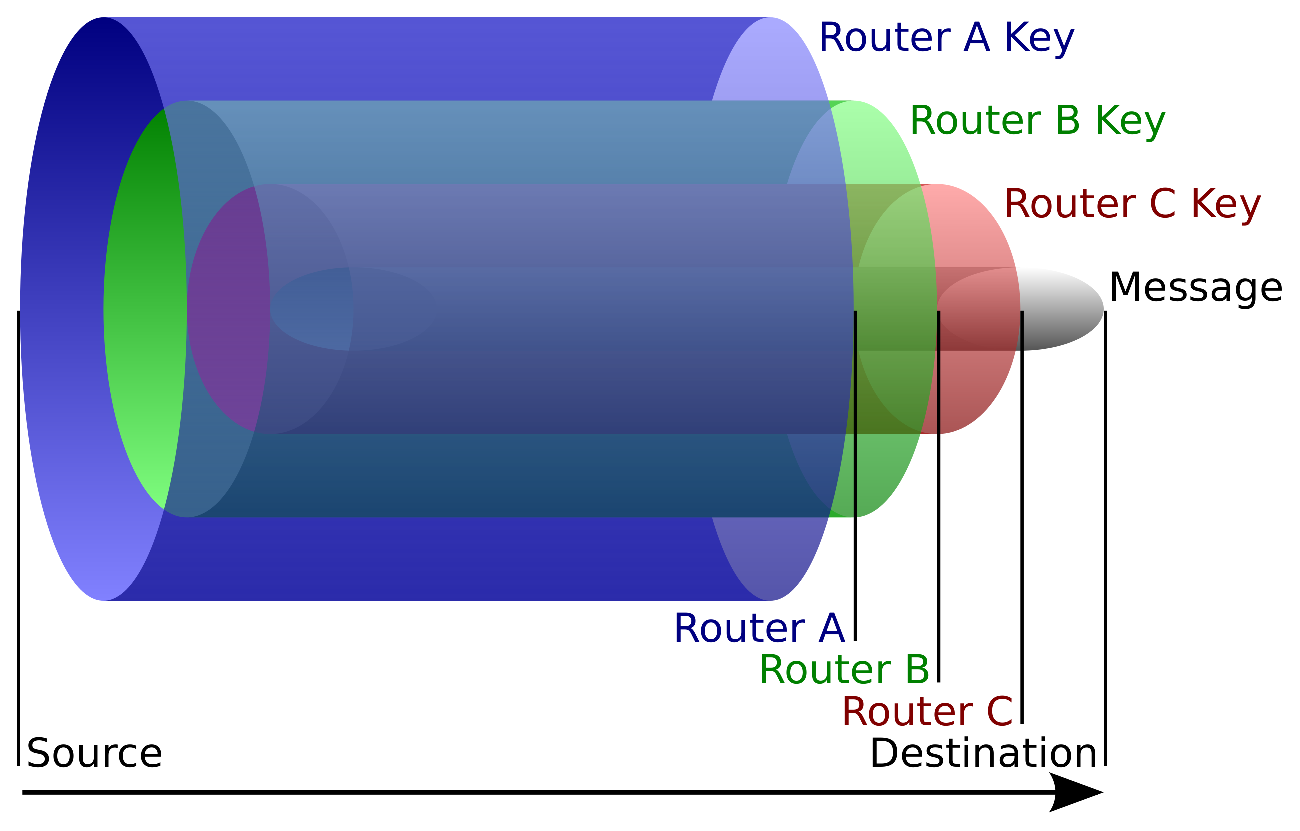
\includegraphics[width=0.5\textwidth]{images/onion-diagram.eps}
	\caption{An example cell and message encryption in an onion routing scheme. Each router ``peals'' off its respective layer of encryption; the final router exposes the final destination.}
\end{figure}

\section{Tor}

Tor is a third-generation onion routing system. It was invented in 2002 by Roger Dingledine, Nick Mathewson, and Paul Syverson of the Free Haven Project and the U.S. Naval Research Laboratory\cite{dingledine2004tor} and is the most popular onion router in use today. Tor inherited many of the concepts pioneered by earlier onion routers and implemented several key changes:\cite{syverson2011peel}\cite{dingledine2004tor}

\begin{itemize}
	\item \textbf{Perfect forward secrecy:} Rather than distributing keys via onion layers, Tor clients negotiate ephemeral symmetric encryption keys with each of the routers in turn, extending the circuit one router at a time. Each router remembers its respective key and can re-encrypts responses as it travels backwards up the circuit to the client, who then unwraps all the layers. These keys are then purged when the circuit is torn down; this achieves perfect forward secrecy, a property that ensures that the session encryption keys will not be revealed if long-term public keys are later compromised.
	\item \textbf{Circuit isolation:} Second-generation onion routers mixed cells from different circuits in realtime, but later research could not justify this as an effective defence against an active adversary\cite{syverson2011peel}. Tor abandoned this in favor of isolating circuits from each other inside the network, although it recycles TCP/IP links between routers.
	\item \textbf{Three-hop circuits:} Previous onion routers used long circuits to provide heavy traffic mixing. Tor removed mixing and fell back to using short circuits of minimal length. With three relays involved in each circuit, the first router (the \emph{guard}) is exposed to the user's IP address. The middle router passes onion cells between the guard and the final router (the \emph{exit}) and its encryption layer exposes it to neither the user's IP nor its traffic. The exit processes user traffic, but is unaware of the origin of the requests. While the choice of middle and exits can be routers can be safely random, the guard must be chosen once and then consistently used to avoid a large cumulative chance of leaking the user's IP to an attacker. This is of particular importance for circuits from hidden services\cite{overlier2006locating}\cite{bauer2007low}.
	\item \textbf{Standardized to SOCKS proxy:} Tor simplified the multiplexing pipeline by transitioning from application-level proxies (HTTP, FTP, email, etc) to a TCP-level SOCKS proxy, which multiplexed user traffic and DNS requests through the onion circuit regardless of any higher protocol. The disadvantage to this approach is that Tor's client software has less capability to cache data and strip identifiable information out of a protocol. The countermeasure was the Tor Browser, a fork of Mozilla's open-source Firefox with a focus on security and privacy. To reduce the risks of users breaking their privacy through Javascript, it ships with the NoScript extension which blocks all web scripts not explicitly whitelisted. The browser also forces all web traffic, including DNS requests, through the Tor SOCKS proxy, provides a Windows-Firefox user agent regardless of the native platform, and includes many sanitization, security, and privacy enhancements not included in native Firefox. The browser also utilizes the Electronic Frontier Foundation's HTTPS Everywhere extension to re-write HTTP web requests into HTTPS whenever possible, providing an additional encryption layer that hides web traffic from exit routers.
	\item \textbf{Directory servers:} Tor introduced a set of trusted directory servers, called directory authorities, to collect, digitally sign, and distribute network information such as the IP addresses and public keys of onion routers. Onion routers mirror the network information from the directories, distributing the bandwidth load. This simplified approach is more flexible and scales faster than the previous flooding approach, but relies on the trust of central directory authorities. Tor ensures that each authority is independently maintained in multiple locations and jurisdictions, reducing the likelihood of an attacker compromising all of them\cite{syverson2011peel}. We describe the contents and format of this network information in section \ref{sec:ConsensusDocs}.
	\item \textbf{Dynamic rendezvous with hidden services:} In previous onion routers, circuits mated at a fixed common node and did not use perfect forward secrecy. Tor introduced a distributed hashtable to record the location of the introduction node for a given hidden service. Following the initial handshake, the server and the client then meet at a different onion router chosen by the client. This approach significantly increased the reliability of hidden services and distributed the communication load across multiple rendezvous points\cite{dingledine2004tor}. We provide additional details on the hidden service protocol in section \ref{sec:HiddenServices} and our motivation for addition infrastructure in section \ref{sec:Motivation}.
\end{itemize}

As of March 2015, Tor has 2.3 million daily users that together generate 65 Gbit/s of traffic. Tor's network consists of nine directory authorities and 6,600 onion routers in 83 countries\cite{TorMetrics}. In a 2012 Top Secret U.S. National Security Agency presentation leaked by Edward Snowden, Tor was recognized as the "the king of high secure, low latency Internet anonymity"\cite{landau2014highlights}\cite{plak2014anonymous}. In 2014, BusinessWeek claimed that Tor was ``perhaps the most effective means of defeating the online surveillance efforts of intelligence agencies around the world.''\cite{TorBusinessWeek}

\subsection{Design}

Tor's design focuses on being easily deployable, flexible, and well-understood. Tor also places emphasis on usability in order to attract more users; more user activity translates to an increased difficulty of isolating and breaking the privacy of any single individual. Tor however does not manipulate any application-level protocols nor does it make any attempt to defend against global attackers. Instead, its threat model assumes that the capabilities of adversaries are limited to observing fractions of Tor traffic, that they can actively delay, delete, or manipulate traffic, that they may attempt to digitally fingerprint packets, that they may run onion routers themselves, and that they may compromise a fraction of other existing routers. Together, most of the assumptions may be broadly classified as traffic analysis attacks. Tor's final focus is defending against these types of attacks\cite{dingledine2004tor}.

\begin{figure}[htdp]
	\begin{minipage}[b]{0.48\linewidth}
		\centering
		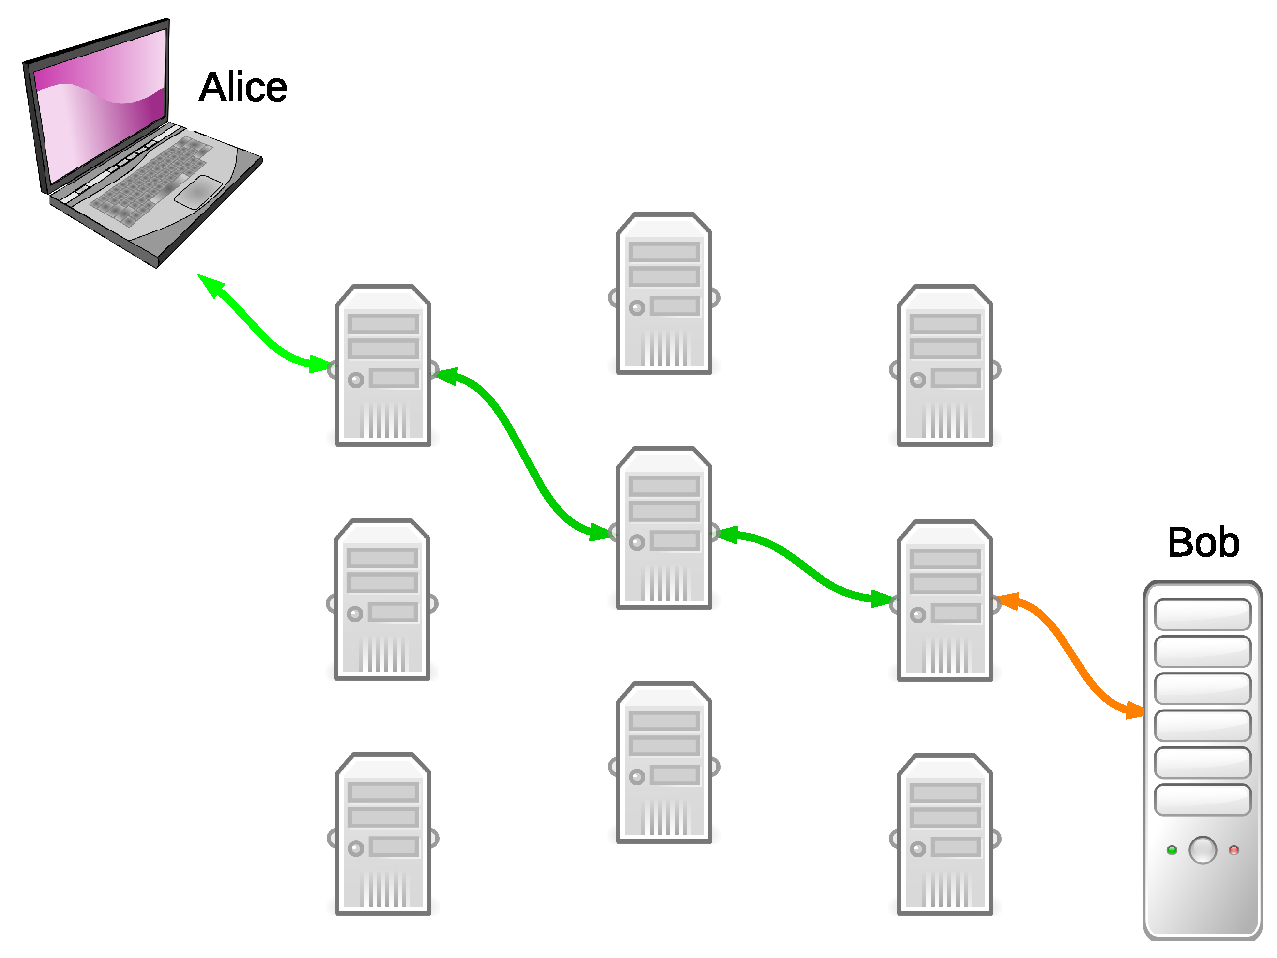
\includegraphics[width=\textwidth]{images/LucidCharts/Tor_Circuit_Orig.pdf}
	\end{minipage}
	\hspace{0.5cm}
	\begin{minipage}[b]{0.48\linewidth}
		\centering
		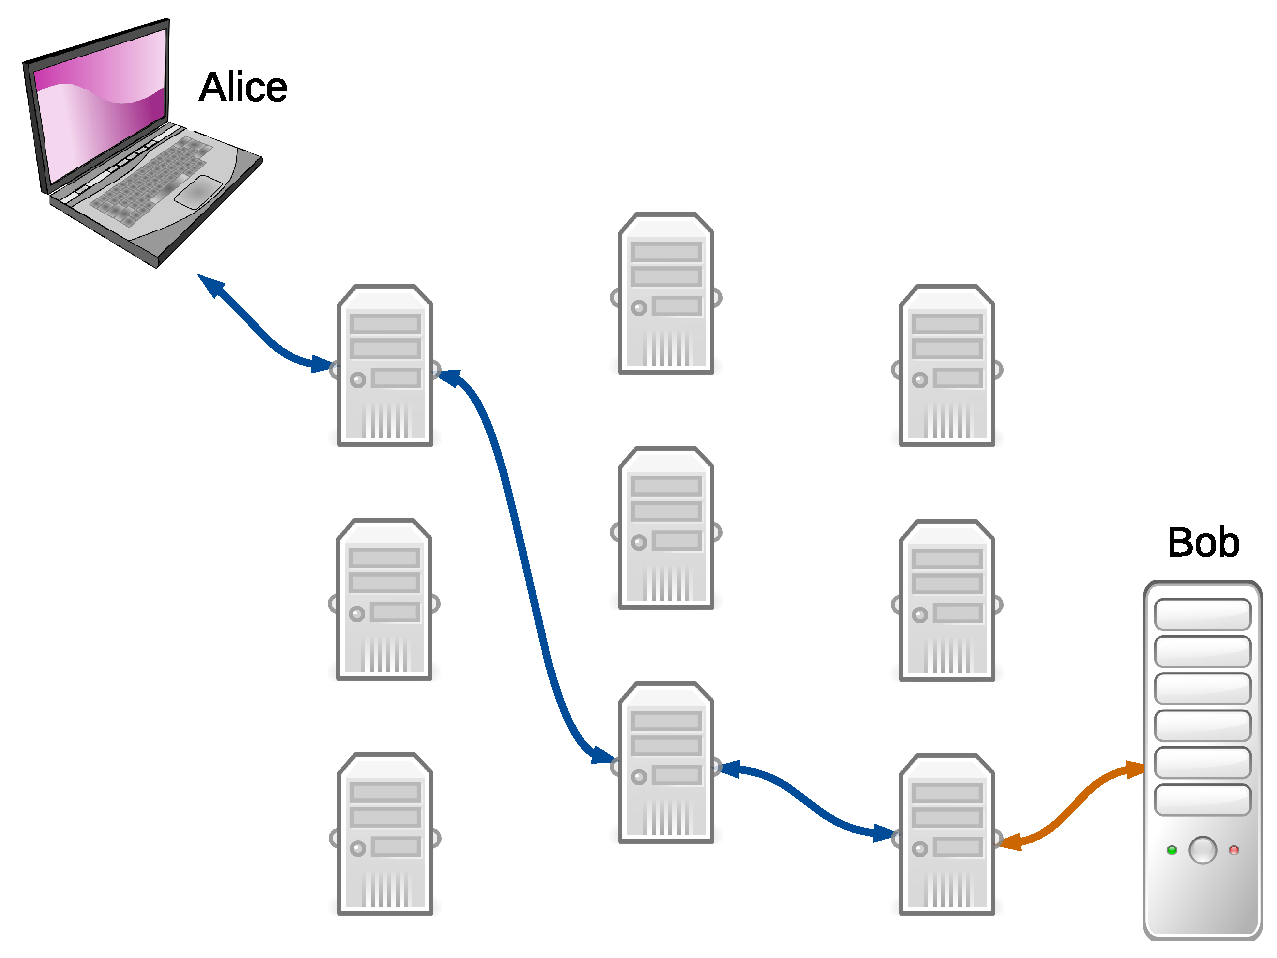
\includegraphics[width=\textwidth]{images/LucidCharts/Tor_Circuit_Change.pdf}
	\end{minipage}
	\caption{Alice communicates privately to Bob through a Tor circuit. Her communication path consists of three routers, an entry, middle, and exit. Although Bob's identity and location is known to Alice, the Tor circuit prevents Bob from knowing Alice's identity or location. At a later time, Alice may construct a different circuit to Bob, giving her a new identity from Bob's perspective. Each encrypted Tor link is shown in green, the final connection from the exit to Bob, shown in orange, is optionally encrypted.}
	\label{fig:torOverview}
\end{figure}

\subsection{Consensus Documents}
\label{sec:ConsensusDocs}

Early mixnets and onion routers either assumed a static network topology or flooded updates across the network. By contrast, Tor's network is maintained by a small set of semi-trusted directory authorities. Periodically, Tor routers upload digitally signed ``descriptors'' to these authorities. A descriptor may contain essential routing numbers, router capabilities, cryptographic keys, bandwidth history, or other information.

Each directory authority maintains an long-term authority key (distinct from its normal identity key if it is a Tor router) and a medium-term signing key. Periodically, each directory authority 

\begin{enumerate}
	\item Aggregates the descriptors into a single ``status vote'' document.
	\item Signs its vote with its signing key.
	\item Exchanges its vote and signature with all other authorities.
	\item Computes a single network status consensus from all the other voting documents.
	\item Signs the network consensus and exchanges the signature with all other authorities.
\end{enumerate}

Once this is complete, the consensus is published and is available for download. If clients have knowledge of the Tor network, they may download the more recent consensus from the directory-mirroring routers. By this system, new routers or changes to existing routers can be propagated to all parties within a very short timeframe. Although routers can optionally publish additional non-essential descriptors, clients and routers typically only need the essential descriptors containing routing information, directory signing keys, and router keys. We discuss the documents containing these descriptors below\cite{TorCollector}\cite{TorDirSpec}:

\subsubsection{cached-certs}

The \emph{cached-certs} document contains the long-term authority identity keys and the medium-term signing keys from each directory authority. The Tor source includes the long-term keys, so all parties can verify the authenticity of the signing keys and in turn the descriptors signed by them. They will believe router descriptors if more than half of the authorities have signed it. Each certificate contains the following fields:

\begin{itemize}
	\item \textbf{fingerprint:} The SHA-1 hash of the identity key.
	\item \textbf{dir-key-published:} The time in UTC when the keys were last published.
	\item \textbf{dir-key-expires:} The time in UTC when the signing keys expire.
	\item \textbf{dir-identity-key:} The identity key, typically a 3072-bit RSA key.
	\item \textbf{dir-signing-key:} The signing key, typically a 2048-bit RSA key.
	\item \textbf{dir-key-crosscert:} The signature of the identity key, made using the signing key.
	\item \textbf{dir-key-certification:} The signature from the identity key of the above fields.
\end{itemize}

\subsubsection{cached-microdesc-consensus}

The \emph{cached-microdesc-consensus} document contains network status information. The document includes a header and then a list of condensed descriptors from each router, called microdescriptors. The header includes the following fields:

\begin{itemize}
	\item \textbf{valid-after} (VA), \textbf{fresh-until} (FU), and \textbf{valid-until} (VU). Three timestamps in UTC, $ \mathrm{VA} < \mathrm{FU} < \mathrm{VU} $. VA and VU specifies the earliest and latest time that these descriptors are valid, respectively. All three values are chosen such that two consensuses overlap: $ \mathrm{consensus}_{x} $ will be considered fresh until $ \mathrm{consensus}_{x+1} $ becomes valid, and then $ \mathrm{consensus}_{x} $ expires when $ \mathrm{consensus}_{x+1} $ is no longer fresh.
	\item \textbf{client-versions} and \textbf{server-versions:} An ascending list of recommended Tor versions for clients and routers, respectively.
	\item A list of directory authorities, each containing:
		\begin{itemize}
			\item \textbf{dir-source:} The authority's nickname, fingerprint, IP address, onion routing port, and directory port.
			\item \textbf{contact:} Optional contact information for the authority operator.
			\item \textbf{vote-digest:} The hash of the authority's status vote document.
		\end{itemize}
\end{itemize}

Following the header, each microdescriptor contains:

\begin{itemize}
	\item \textbf{r:} The router's nickname, fingerprint, time of last restart, IP address, onion routing port, and directory port.
	\item \textbf{m:} The SHA-256 hash of the router's microdescriptor. This also includes its entries in the \emph{cached-microdescs} document (discussed below).
	\item \textbf{s:} A list of the router's status flags, as given by the directory authorities. Common examples include Running, Valid, Fast, Guard, Stable, and Exit.
	\item \textbf{v:} The version of the Tor software that the router is running.
	\item \textbf{w:} The estimated bandwidth that this router is capable of. This value is determined by speed tests from bandwidth authorities, who are a subset of the directory authorities.
\end{itemize}

\subsubsection{cached-microdescs}

The \emph{cached-microdescs} document contains cryptographic keys from each Tor router. Each entry contains:

\begin{itemize}
	\item \textbf{onion-key:} The router's public RSA key.
	\item \textbf{ntor-onion-key:} The router's public Curve25519 key.
	\item \textbf{family:} The fingerprint of routers also under the operator's administration; Tor clients will not construct circuits through any routers that have the same family or that are in the same /16 IPv4 block.
	\item \textbf{id:} The router's fingerprint.
\end{itemize}

\subsection{Hidden Services}
\label{sec:HiddenServices}

Although Tor's primary and most popular use is for privacy-enhanced access to the traditional Internet, Tor also supports \emph{hidden services} -- anonymous servers hosting services such as websites, marketplaces, or chatrooms. These servers intentionally mask their IP addresses through Tor circuits and thus cannot normally be accessed outside the context of Tor. In contrast to Tor-anonymized web requests where the client is anonymous but the server is known, Tor hidden services provide bidirectional anonymity where both parties remain anonymous and never directly communicate with one another\cite{nicolussi2011human}.

Hidden services are known by their special domain name, which uses the .onion top-level domain (TLD). The Tor software considers this TLD a special case and does not attempt to resolve it on the Internet DNS, but rather through the Tor network. Hidden service addresses are algorithmically generated from the server's public RSA key; the address is the first 16 bytes of the base32-encoded SHA-1 hash of the server's RSA key. This builds a publicly-confirmable one-to-one relationship between the public key and its address and allows hidden services to be referenced by their address in a distributed environment.

Let Bob be a hidden service. At startup, Bob randomly selects several router and builds Tor circuits to them. He then creates a hidden service descriptor, consisting of his public key $ B_{K} $ and a list of these routers. He signs the descriptor and sends a distributed hashtable within the Tor network, enabling the routers he chose to act as his \textit{introduction points}. When Alice, a Tor client, obtains Bob's hidden service address though a backchannel, she queries this hashtable for Bob's address. Once she obtains Bob's hidden service descriptor, she then builds a circuit to one of the introduction points. Simultaneously, Alice also selects and builds a circuit to another relay, $ R_{A} $. She encrypts $ R_{A} $ and a nonce with $ B_{K} $ and gives the result to $ R_{A} $. Bob decrypts the message and builds a circuit to $ R_{A} $ (for security reasons, he uses the same guard router \cite{bauer2007low}\cite{overlier2006locating}) and sends the nonce to Alice. Alice can then confirm Bob's authenticity and the two can begin communication over six Tor nodes: three established by Alice and three by Bob.

\begin{figure}[htdp]
	\begin{minipage}[b]{0.48\linewidth}
		\centering
		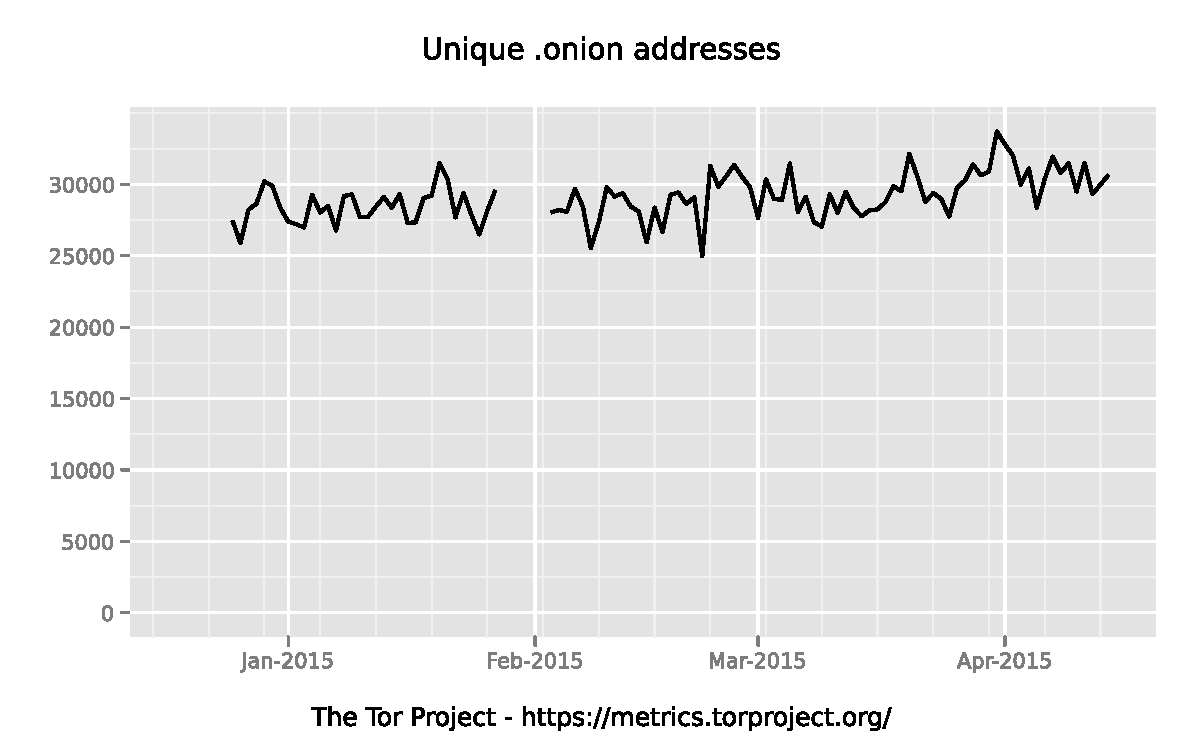
\includegraphics[width=\textwidth]{images/Tor/onion_2014-10_2015-04.pdf}
		\caption{The number of unique .onion addresses seen in Tor's distributed hashtable between January through April 2015\cite{TorMetrics}\cite{kadianakis2015extrapolating}.}
	\end{minipage}
	\hspace{0.5cm}
	\begin{minipage}[b]{0.48\linewidth}
		\centering
		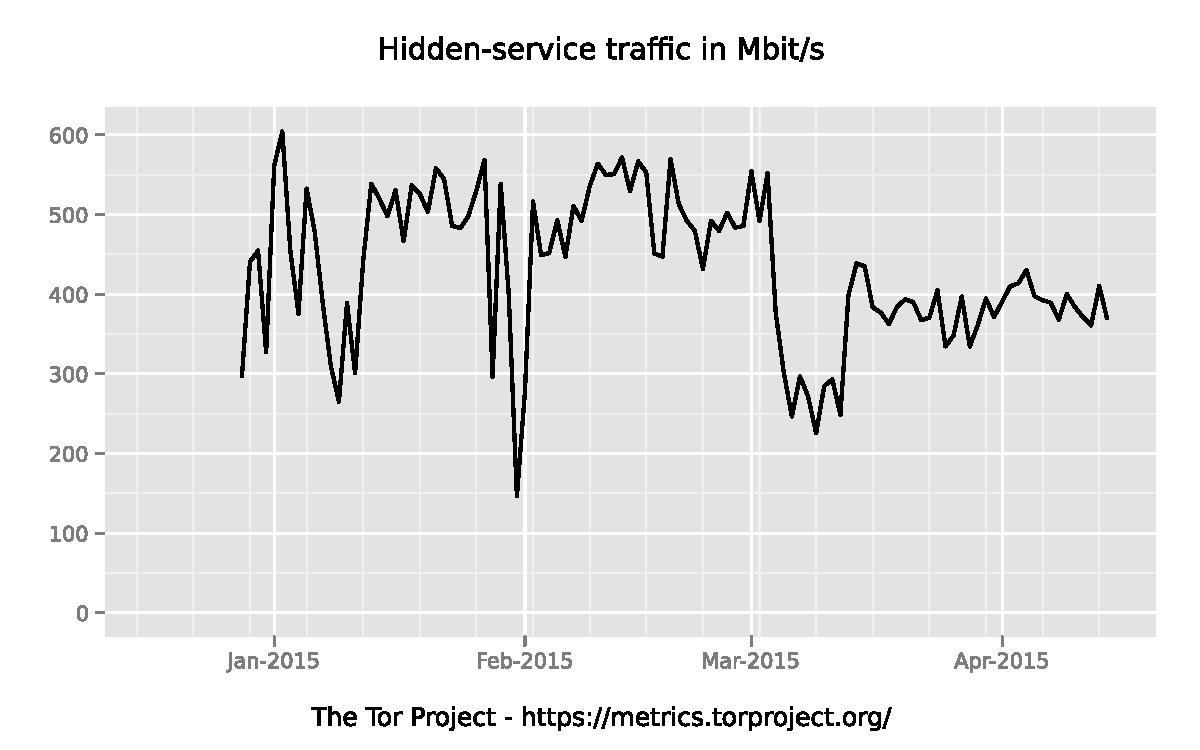
\includegraphics[width=\textwidth]{images/Tor/onionbw_2014-11_2015-04.pdf}
		\caption{The amount of traffic generated by hidden services between January through April 2015\cite{TorMetrics}\cite{kadianakis2015extrapolating}.}
	\end{minipage}
\end{figure}

\newpage

\section{Motivation}
\label{sec:Motivation}

Tor hidden service addresses are distributed and globally collision-free, but there is a strong discontinuity between the address and the service's purpose. For example, a visitor cannot determine that \url{3g2upl4pq6kufc4m.onion} is the DuckDuckGo search engine without visiting the hidden service. Generally speaking, it is currently impossible to categorize or fully label hidden services in advance. Over time, third-party directories -- both on the Clearnet and Darknet -- have appeared in attempt to counteract this issue, but these directories must be constantly maintained and the approach is neither convenient nor does it scale well. Given the approximetly 25,000 hidden services on the Tor network, this suggests the strong need for a more complete and reliable solution to solve the usability issue.

\section{Contributions}

Our contribution to this problem is five-fold:

\begin{itemize}
	\item We enable hidden service operators to construct a strong association between a unique human-meaningful domain name and their hidden service address.
	\item We described a distributed DNS database that is tamper-proof, self-healing, resistant to node compromise, and provides authenticated denial-of-existence.
	\item We provide OnioNS as a plugin for the existing Tor network, rather than introduce a new network. This simplifies our assumptions and largely reduces our threat model to attack vectors already well-understood on the Tor network.
	\item We enable Tor clients to verify the authenticity of a domain name against its corresponding hidden service address with minimal data transfers in a single query.
	\item We preserve the anonymity of both the hidden service and the privacy of Tor clients connecting to it.
\end{itemize}

To the best of our knowledge, this is the first alternative DNS for Tor hidden services which is distributed, secure, and usable at the same time.
